\section{Results}
\label{sec:results}

\begin{figure*}[t]
\centering
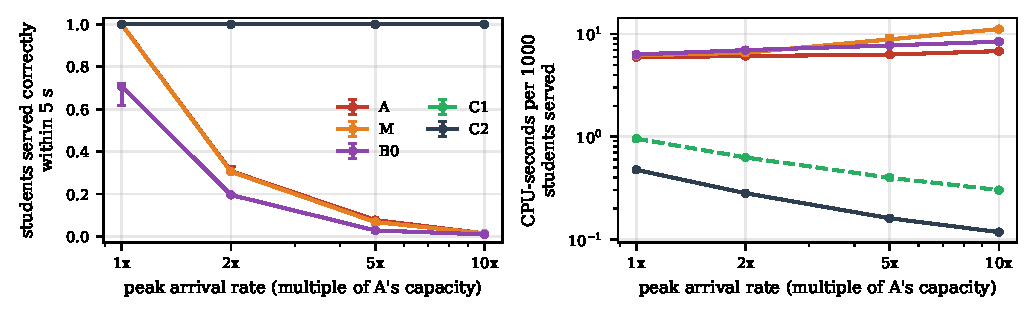
\includegraphics[width=\textwidth]{figures/core.pdf}
\caption{Left: share of students who received their correct result within
\SI{5}{s} of their first request after release. Right: CPU-seconds used by all
containers per \num{1000} students served (log scale). Medians of 3 runs with
95\% bootstrap intervals. C1 (dashed) and C2 overlap at 100\%.}
\label{fig:core}
\end{figure*}

\begin{table}[t]
\caption{Students served correctly within 5\,s (\%) and CPU-seconds per 1000 served, median of 3 runs}
\label{tab:core}
\centering
\footnotesize
\setlength{\tabcolsep}{3pt}
\begin{tabular}{@{}lrrrrrrrr@{}}
\toprule
 & \multicolumn{2}{c}{1$\times$} & \multicolumn{2}{c}{2$\times$} & \multicolumn{2}{c}{5$\times$} & \multicolumn{2}{c}{10$\times$} \\
\cmidrule(lr){2-3} \cmidrule(lr){4-5} \cmidrule(lr){6-7} \cmidrule(lr){8-9}
Design & 5\,s \% & CPU & 5\,s \% & CPU & 5\,s \% & CPU & 5\,s \% & CPU \\
\midrule
A & 100.0 & 5.9 & 30.8 & 6.1 & 7.7 & 6.3 & 1.4 & 6.8 \\
M & 100.0 & 6.2 & 30.5 & 6.5 & 6.8 & 8.9 & 1.4 & 11.1 \\
B0 & 70.8 & 6.3 & 19.6 & 6.9 & 2.8 & 7.7 & 0.9 & 8.4 \\
C1 & 100.0 & 1.0 & 100.0 & 0.6 & 100.0 & 0.4 & 100.0 & 0.3 \\
C2 & 100.0 & 0.5 & 100.0 & 0.3 & 100.0 & 0.2 & 100.0 & 0.1 \\
\bottomrule
\end{tabular}
\end{table}


\subsection{RQ1: Architecture and cost}
\label{sec:rq1}

Table~\ref{tab:core} and Fig.~\ref{fig:core} compare the five designs from
1$\times$ to 10$\times$ the calibrated capacity of design~A. In this grid
students neither refresh nor look again, so every design faces exactly the same
requests; the other grids use the full student model. No run in this grid
returned a wrong, stale or missing result, no container crashed, and the load
generator never saturated.

\textbf{Building pages on request does not survive the surge.} Design~A served
every student within \SI{5}{s} at 1$\times$ (98.8\% within \SI{2}{s}), but only
30.8\% at 2$\times$, 7.7\% at 5$\times$ and 1.4\% at 10$\times$. Many students
never received a result before giving up: 78.4\% were served at all at
2$\times$, 39.9\% at 5$\times$ and 20.6\% at 10$\times$.

\textbf{Mirrors do not help.} Splitting the same two CPUs into two independent
copies (M) matched A at 1$\times$ and 2$\times$ (100\% and 30.5\% within
\SI{5}{s}) and fell behind it at higher load: 29.8\% of students were served at
all at 5$\times$ (A: 39.9\%) and 13.1\% at 10$\times$ (A: 20.6\%). Each mirror
has half the budget, so both overload at the same multiple. M also used more
CPU per student served than A: 1.04 times as much at 1$\times$ and 1.64 times
at 10$\times$.

\textbf{A cold cache is worse than no cache.} Cache-aside without pre-warming
(B0) was below A at every load, with 70.8\% of students served within
\SI{5}{s} even at 1$\times$. Every student looks up a different roll number
once, so almost every request misses the cache: B0 issued one database query
per student at 1$\times$, exactly as A did, while giving \num{0.5} of its two
CPUs to Redis. Section~\ref{sec:rq4} examines these misses.

\textbf{Pre-computed results serve the whole surge.} C1 (results pre-computed
into Redis) and C2 (one static file per student behind Nginx) served every
student at every multiple; C1 served all of them within \SI{2}{s} and C2 at
least 99.97\% within \SI{5}{s}, with 99th-percentile latencies below
\SI{0.7}{ms}. Their capacity lies beyond what our generator can offer: C1's
calibration stopped at \CapCOne\ students/s, where the generator saturated,
33.6 times the capacity of A. The few C2 students served later than
\SI{5}{s} (63 of \num{404723} across its 12 runs) all asked within the first
\SI{31}{ms} after the announced time, before the release flag file appeared,
were told ``not released'', and received their result at their next reload.
C1 checks the release time in the application and had no such case.

\textbf{Cost.} Pre-computation also costs far less to serve. Design~A used
\num{5.9} to \num{6.8} CPU-seconds per \num{1000} students served; C1 used
\num{0.96} at 1$\times$ falling to \num{0.30} at 10$\times$, and C2 \num{0.48}
falling to \num{0.12}, because fixed costs such as the idle back-office
database are shared by more students as load rises. Per
student served, A needed 12.5 times C2's CPU at 1$\times$ and 57.8 times at
10$\times$. The price is a preparation step before release: pre-computing all
\num{200000} results took a median of 6.9--\SI{7.0}{s} for C1 and
9.4--\SI{9.8}{s} for C2 across load levels.

\textbf{Page cost.} The \SI{5}{ms} page-building cost is an assumption, so we
repeated A and B0 at the same load as 2$\times$ with \SI{2}{ms} and \SI{0}{ms}.
Both then served at least 99.8\% of students within \SI{5}{s}: the page cost
decides how much load a database-backed portal can take. The cost order did
not change. Per student served, A used 2.6 (\SI{0}{ms}) to 9.7 (\SI{2}{ms})
times the CPU of C2, and B0 always used more than A (1.12 against 0.73
CPU-seconds per \num{1000} at \SI{0}{ms}, 3.05 against 2.73 at \SI{2}{ms}).

\textbf{Answer to RQ1.} Designs that build each page when it is requested fail
at twice design~A's capacity (A and M) or already at its capacity (B0), and
neither mirrors nor a cold cache helps. Pre-computing results before release
served 10$\times$ that load without loss, at 12.5--57.8 times less CPU per
student than design~A, after less than \SI{10}{s} of preparation.

\subsection{RQ2: Waiting rooms}
\label{sec:rq2}

\begin{table*}[t]
\caption{Waiting rooms at 5$\times$ load with refreshing students (median of 3 runs). Wait: from first request after release until admitted. $\tau$: Kendall's rank correlation between arrival and admission order (1 = first-come-first-served). Refresh penalty: median extra wait of students who pressed refresh.}
\label{tab:wr}
\centering
\footnotesize
\begin{tabular}{@{}llrrrrrrrrr@{}}
\toprule
Backend & Waiting room & \multicolumn{3}{c}{Served correctly (\%)} & Still waiting & Wait p50 & Wait p95 & $\tau$ (early arrivals) & Refresh penalty & CPU s / 1000 \\
\cmidrule(lr){3-5}
 & & 5\,s & 10\,s & at all & at end (\%) & (s) & (s) & & (s) & \\
\midrule
A & none & 3.5 & 6.1 & 43.3 & 0.0 & 0.2 & 17.5 & 0.09 & -- & 8.3 \\
A & fifo, token & 2.0 & 4.1 & 36.8 & 52.2 & 40.6 & 102 & 0.79 & 20.1 & 11.6 \\
A & fifo, naive & 1.9 & 3.7 & 41.9 & 58.1 & 59.5 & 105 & 0.60 & 36.8 & 8.2 \\
A & random, token & 2.3 & 4.4 & 34.2 & 52.5 & 38.2 & 104 & 0.01 & 17.9 & 12.6 \\
A & random, naive & 1.9 & 3.8 & 41.8 & 58.1 & 59.8 & 105 & -0.01 & 37.2 & 8.3 \\
\midrule
C1 & none & 100.0 & 100.0 & 100.0 & 0.0 & 0.0 & 0.0 & 0.25 & -- & 0.4 \\
C1 & fifo, token & 99.7 & 100.0 & 100.0 & 0.0 & 0.0 & 0.1 & 0.16 & 0.0 & 0.8 \\
C1 & fifo, naive & 99.7 & 100.0 & 100.0 & 0.0 & 0.0 & 0.0 & 0.15 & 0.0 & 0.8 \\
C1 & random, token & 99.7 & 100.0 & 100.0 & 0.0 & 0.0 & 0.1 & 0.13 & 0.0 & 0.8 \\
C1 & random, naive & 99.6 & 100.0 & 100.0 & 0.0 & 0.0 & 0.1 & 0.13 & 0.0 & 0.8 \\
\bottomrule
\end{tabular}
\end{table*}


Table~\ref{tab:wr} compares A and C1 alone with the same backends behind our
waiting room, at 5$\times$ with our default, refreshing students. A run ends
\SI{135}{s} after release: the \SI{90}{s} surge and \SI{45}{s} to finish.

\textbf{In front of an overloaded backend, the waiting room turns failures
into waiting.} It admits students at 80\% of A's capacity, about 179 per
second, so letting in all of the roughly \num{37500} students takes about 3.5
minutes, longer than our run. Within the run it served slightly fewer students
than A alone: 41.9\% (first come, first served) and 41.8\% (lottery) with
naive tickets, and 36.8\% and 34.2\% with tokens, against 43.3\%. The
difference is in the rest. A's unserved students had given up; 52--58\% of the
waiting room's students were still in the queue when the run ended. Waiting
was long: the median student waited 38--\SI{60}{s} to be admitted, and only
3.7--4.4\% were served within \SI{10}{s} (A alone: 6.1\%).

\textbf{Tickets.} With naive tickets, a student who pressed refresh while
queued lost their place and rejoined at the back. Each lost ticket was later
skipped as abandoned: about \num{15700} per run, against 27 to 100 with tokens.
Pressing refresh cost a median of 37~seconds of extra waiting with naive
tickets and 18--\SI{20}{s} with tokens. With naive tickets fewer students
reached A within the run, which received only 0.46 requests per student. But, as with impatient
students in Section~\ref{sec:refresh}, admitted students who ran out of
patience refreshed straight at A, which received 1.55--1.72 requests per
student and spent 11.6--12.6 CPU-seconds per \num{1000} students served,
against 8.3 without a waiting room.

\textbf{Fairness.} For students who arrived before release, first come, first
served with tokens kept them in arrival order (Kendall's $\tau=0.79$ between
arrival and admission order). Naive tickets lowered this to 0.60, because
refreshing students went to the back. The lottery gave $\tau$ close to 0 by
design ($0.01$ and $-0.01$), and so did A alone ($0.09$): without a queue,
which early student gets through is close to random.

\textbf{In front of a fast backend, the waiting room only adds cost.} C1 alone
served every student within \SI{5}{s}. Behind the waiting room, 99.6--99.7\%
were served within \SI{5}{s} and all within \SI{10}{s}, nobody waited more
than \SI{0.1}{s} at the 95th percentile, and the CPU used per \num{1000}
students rose from 0.4 to 0.8 CPU-seconds, because every request also passes
through the waiting room.

\textbf{Longer runs.} Because so many students were still queued, we ran D-A
with first come, first served again with \SI{240}{s} more for the queue to
empty (a \SI{330}{s} run). With naive tickets it then served 98.3\% of
students, against 43.3\% for A alone, whose unserved students had all given
up; but the median student waited \SI{121}{s} to be admitted (95th percentile
\SI{282}{s}). In our model, queued students wait up to 10 minutes; real
students may leave sooner. With tokens it served only 74.5\%: admitted
students who ran out of patience refreshed straight at A, which received 3.21
requests per student instead of 1.07.

\textbf{Answer to RQ2.} At 5$\times$ our waiting room served almost every
student in the end, against fewer than half without it, but only after waits
of minutes. It kept arrival order only with first come, first served and
tokens. Tokens protect a student who presses refresh, but without a limit on
admitted students they also let impatient students overload the backend, and
then it served fewer students. In front of a backend that can take the load, a
waiting room adds cost and delay for no gain.

\subsection{RQ3: Correctness}
\label{sec:rq3}

\begin{table}[t]
\caption{Correctness at 1$\times$ load, totals over 3 runs. Top: corrections for 1\% of students published 30\,s after release; \emph{answers} are those given to corrected students after that time. Bottom: release with only 90\% of results pre-computed.}
\label{tab:correct}
\centering
\footnotesize
\setlength{\tabcolsep}{3pt}
\begin{tabular}{@{}lp{2.9cm}rrr@{}}
\toprule
Design & Condition & Answers & Stale & Last stale (s) \\
\midrule
A & database read every time & 90 & 1 & 0.07 \\
B0 & cache entries deleted & 92 & 0 & -- \\
B0 & no invalidation (TTL 10 min) & 94 & 4 & 10.89 \\
C1 & Redis entries rewritten & 90 & 1 & 0.07 \\
C2 & files rewritten, Nginx cache 1\,s & 90 & 1 & 0.07 \\
C2 & files rewritten, Nginx cache 30\,s & 90 & 5 & 13.69 \\
\midrule
Design & & Written late & Took (s) & Missing \\
\midrule
C1 & release with 90\% ready & 20,058 & 0.08 & 1 \\
C2 & release with 90\% ready & 20,058 & 1.63 & 0 \\
\bottomrule
\end{tabular}
\end{table}


Table~\ref{tab:correct} shows the correctness runs, all at 1$\times$. No design
returned a wrong result, that is, another student's marks or marks that were
never published.

\textbf{Corrections.} \num{1994} students (1\%) receive a revised result
\SI{30}{s} after release. Most students look only once, and most had looked
before the correction, so corrected students received only about 90 answers
after it in the three runs of each configuration. The results:
\begin{itemize}
\item Reading the database every time (A), deleting the cache entry (B0) or
rewriting the stored result (C1) gave at most one stale answer. It came
\SI{0.07}{s} after the correction time, while the correction was still being
written; writing it finished within \SI{0.19}{s} in every run.
\item Without cache invalidation, B0 kept serving the old result: 4 stale
answers, the last one \SI{10.89}{s} after the correction. These entries stay
stale until their 10-minute lifetime ends.
\item C2 rewrote the files, but Nginx kept serving the old ones from its cache
of open files. With that cache valid for \SI{30}{s}, students got 5 stale
answers, the last \SI{13.69}{s} after the correction. With \SI{1}{s}, there was
one, again while the correction was being written.
\end{itemize}

\textbf{Early release.} When only 90\% of results were pre-computed at
release, C1 wrote the remaining \num{20058} within \SI{0.08}{s} and C2 within
\SI{1.63}{s}. Across three runs each, one student was told ``not found'' for a
roll number that exists (C1). The harm is small here only because our
preparation is fast: students who ask before their result is written get
``not found'', so a slower pipeline would leave more of them without a result
for longer.

\textbf{Answer to RQ3.} Under load, no design returned wrong results. Stale
results came from copies that were not updated when a result was corrected: a
cache without invalidation and Nginx's file cache. Deleting or rewriting the
copy, and keeping file caches short, avoided them. Few students saw stale
results only because few looked again after the correction; a correction
published while students are still looking would reach more of them.

\subsection{RQ4: Cache misses and refreshes}
\label{sec:rq4}

\begin{figure*}[t]
\centering
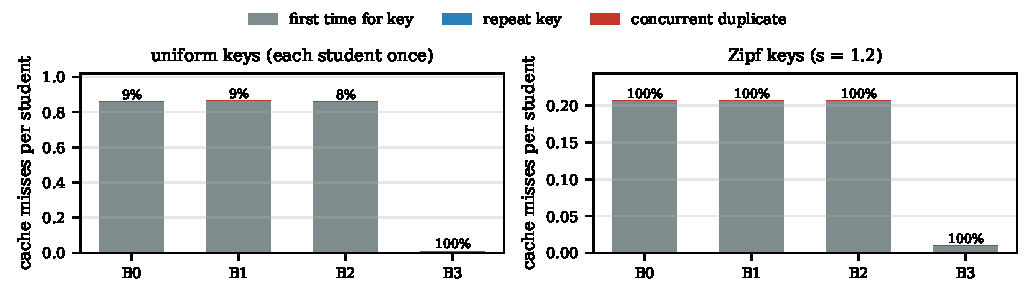
\includegraphics[width=\textwidth]{figures/cache.pdf}
\caption{Cache misses per student for the four cache-aside designs at
2$\times$, by kind (medians of 3 runs). The number above each bar is the share
of students served correctly within \SI{5}{s}.}
\label{fig:cache}
\end{figure*}

Fig.~\ref{fig:cache} breaks down the cache misses of B0--B3 at 2$\times$. Each
miss is one of three kinds: the first request for that roll number, a repeat
request after the entry expired, or a duplicate that arrives while another
request for the same roll number is already filling the cache. Only the last
kind is a stampede, and only it can be helped by request coalescing (B1) or
early recomputation (B2).

\textbf{Per-student keys do not stampede.} When every student looks up a
different roll number, B0 missed 0.86 times per student, and every miss was the
first request for its key: there were no repeats and no duplicates. B1 had
nothing to coalesce and B2 never refreshed an entry early, in any run, so both
did as badly as B0, serving 8.9\%, 8.9\% and 8.5\% of students within
\SI{5}{s}. Filling the cache before release (B3) removed almost every miss.
The few left (0.009 per student) were for mistyped roll numbers, which the
filled cache does not contain. B3 served every student within \SI{5}{s}, using
0.71 CPU-seconds per \num{1000} students against B0's 6.27.

\textbf{Shared keys.} When roll numbers follow a Zipf law, many students ask
for the same few results. Misses fall to 0.21 per student and B0 already
serves everyone within \SI{5}{s}. Even then, only 2 to 3 misses per run were
duplicates, and B1 coalesced a median of 4 requests per run.

\textbf{Answer to RQ4 (caches).} Cache-aside's weakness on result day is not a
stampede. Almost every miss is the first request for a student's result, so
stampede defences have nothing to do; only filling the cache before release
helps.

\subsubsection{Refreshing students}
\label{sec:refresh}

\begin{figure*}[t]
\centering
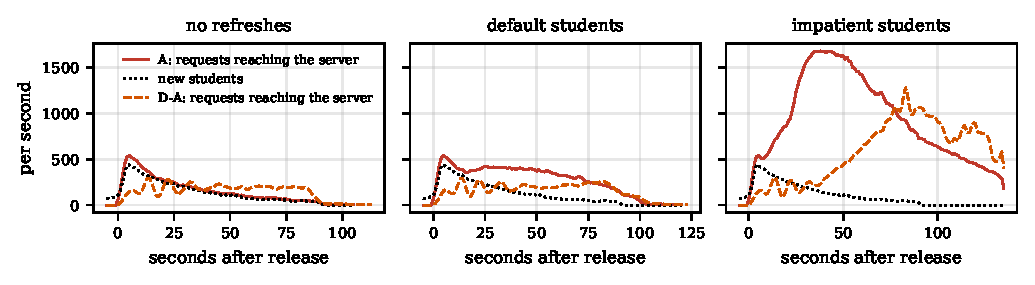
\includegraphics[width=\textwidth]{figures/refresh.pdf}
\caption{Requests reaching the server each second (3-second moving average) for
design~A alone (solid) and behind a waiting room (D-A, dashed) at 2$\times$,
against new students arriving (dotted). One run per behaviour.}
\label{fig:refresh}
\end{figure*}

We ran design~A, alone and behind a waiting room (D-A), at 2$\times$ with three
kinds of students: ones who never refresh, our default students
(Fig.~\ref{fig:student}), and impatient ones who wait only 3--\SI{8}{s},
refresh with probability 0.9--0.95 and pause only 0.5--\SI{2}{s}.
Fig.~\ref{fig:refresh} shows one run of each.

\textbf{Refreshing helps one student and hurts the crowd.} Without refreshes,
A received 1.17 requests per student, served 53.7\% of students within
\SI{10}{s} and 77.7\% at all, and failed requests fell below 1\% (for ten
seconds in a row) \SI{48}{s} after release. With default students it received
2.23 requests per student: more students were served in the end (88.1\%),
because they kept trying, but fewer within \SI{10}{s} (32.7\%), and failures
lasted until \SI{92}{s}. Impatient students
sent 8.65 requests each. Their refreshes kept A overloaded long after new
students stopped arriving (Fig.~\ref{fig:refresh}, right): failures never
dropped below 1\% for ten seconds before the end of any of the three runs, and
only 22.1\% of students were served.

\textbf{A waiting room limits admissions, not requests.} With patient
students, the waiting room kept the load on A close to one request per student
(1.09 without refreshes, 1.32 with default students, against A's 1.08 and
2.14) and served more students in the end: 91.9\% and 97.5\%. The price was
waiting: only about 11\% were served within \SI{10}{s}. With impatient students
it did not protect A. An admitted student may use the backend for
\SI{60}{s}, and in our configuration the waiting room limits neither how many
admitted students are active at once nor how many requests each one sends.
Admitted students who ran out of patience refreshed straight at A, which
received 5.30 requests per student; 46.4\% of students were served, against
22.1\% without the waiting room.

\textbf{Answer to RQ4 (refreshes).} Compared with students who never refresh,
our default students almost doubled the requests per student (2.23 against
1.17) and impatient ones sent 7.4 times as many, and with impatient students an
unprotected portal did not recover within the run. A waiting room kept the load near one request
per student and served more students overall, at the cost of longer waits, but
only while admitted students behaved; it also needs a limit on what each
admitted student may send.
